\subsection{Faust - Processing Layer} \label{sec:faust}
\subsubsection{Introduzione}
\paragraph*{Premessa} 

Per soddisfare il requisito opzionale del calcolo del punteggio di salute, si è scelto di utilizzare Faust, una libreria \textit{Python}\textsubscript{\textit{G}} ispirata al modello di \textit{Kafka}\textsubscript{\textit{G}} Streams. Faust facilita l'elaborazione di flussi di dati distribuiti in tempo reale, rendendola ideale per questo caso d'uso.
Offre un'interfaccia di alto livello che astrae le complessità di \textit{Kafka}\textsubscript{\textit{G}}, rendendo la raccolta dati semplice e intuitiva.
Inoltre Faust è progettato per essere scalabile e può essere utilizzato per gestire grandi volumi di dati.

\paragraph*{Faust \& Schema Registry} 
Faust deserializza i messaggi dei topic in conformità allo schema definito nello Schema Registry. Qualora si riscontrino messaggi non conformi, essi vengono eliminati. I messaggi validi vengono successivamente processati e instradati verso un topic dedicato all'interno di Kafka.

La gestione della connessione allo Schema Registry è integrata in Faust. Dopo aver fornito l'indirizzo dello Schema Registry nella configurazione dell'applicazione Faust, Faust stesso si occupa di validare i messaggi in base allo schema registrato per il relativo topic.

\paragraph*{Calcolo del Punteggio}
Il punteggio di salute rappresenta un indicatore sintetico del benessere generale di una città, misurandolo in base a diversi aspetti chiave. In questo caso, le tre tipologie di misurazioni considerate sono:
\begin{itemize}
    \item Temperatura;
    \item Umidità;
    \item Livello di polveri sottili (PM10).
\end{itemize}

Il calcolo del punteggio avviene in due fasi:
\begin{enumerate}
    \item \textbf{Incrementi}: 
    \begin{itemize}
        \item A intervalli regolari, si calcolano incrementi al punteggio di salute basandosi sulle misurazioni acquisite nell'intervallo precedente.
        \item Ciascuna tipologia di misurazione ha un suo algoritmo di calcolo dell'incremento, basato su soglie predefinite di benessere.
    \end{itemize}
    \item \textbf{Punteggio Finale}:
    \begin{itemize}
        \item Il punteggio di salute finale si ottiene sommando gli incrementi calcolati per le tre tipologie di misurazioni.
        \item Punteggi più alti indicano un minore stato di benessere, con la necessità di interventi per migliorare la qualità della vita.
    \end{itemize}
\end{enumerate}


\subsubsection{Componenti Faust \& Processing Layer}
\begin{itemize}
    \item \textbf{Applicazione Faust:}
    \begin{lstlisting}[style=code]
        faust.App(<nome_app>, broker=<broker_kafka>)
    \end{lstlisting} 
    \begin{itemize}
        \item Un'applicazione Faust è un \textit{programma}\textsubscript{\textit{G}} \textit{Python}\textsubscript{\textit{G}} che elabora flussi di dati in tempo reale da \textit{Kafka}\textsubscript{\textit{G}}.
        \item \textbf{nome\_app}: Identifica l'applicazione, coincide con il \textit{ConsumerGroup} di Kafka.
        \item \textbf{broker\_kafka}: Indirizzo del \textit{broker}\textsubscript{\textit{G}} \textit{Kafka}\textsubscript{\textit{G}} (hostname:porta).
        \item Importante configurare l'applicazione con l'indirizzo dello Schema Registry per garantire a la validazione e deserializzazione dei messaggi.
    \end{itemize}
    \item \textbf{Topic:}
    \begin{lstlisting}[style=code]
        app.topic(<nome_topic>, value_type=<tipo_dato>)
    \end{lstlisting}  
    \begin{itemize}
        \item \textbf{nome\_topic}: Nome del topic \textit{Kafka}\textsubscript{\textit{G}} a cui iscrivere l'app Faust.
        \item \textbf{tipo\_dato:} Classe che rappresenta il tipo di dato del topic (es. FaustMeasurement).
        \item Nel caso si voglia aggiungere altri topic da cui consumare dati basterà aggiungerne prima del parametro value\_type separati da virgole.
    \end{itemize}
    \item \textbf{Tipo di dato atteso:}
     \begin{lstlisting}[style=code]
        class FaustMeasurement(faust.Record, serializer='json')
    \end{lstlisting}  
    \begin{itemize}
        \item È una classe che eredita da \textbf{faust.Record}.
        \item \textbf{faust.Record} è una classe fornita dalla libreria Faust che semplifica la definizione di record per la rappresentazione dei dati in streaming.
        \item Rappresenta una singola misurazione proveniente da un \textit{sensore}\textsubscript{\textit{G}}. Viene usata nella applicazione Faust per definire il tipo di dati atteso nei topic \textit{Kafka}\textsubscript{\textit{G}}.
    \end{itemize}
    \item \textbf{Modello per il calcolo del punteggio di salute:}:
    \begin{itemize}
        \item \textbf{Processore di misurazioni}: 
        Tramite il \textit{pattern}\textsubscript{\textit{G}} \textit{Object Adapter} e l'interfaccia \textit{Processor} l'app faust invia le misurazioni ottenute dai topic al modello per il calcolo del punteggio di salute che verrà adattato come \textit{Processor.}
    \end{itemize}
    \item \textbf{Agente di elaborazione}: 
    \begin{lstlisting}[style=code]
        @app.agent(<topic>).
    \end{lstlisting}  
    \begin{itemize}
        \item Funzioni asincrone che elaborano i dati dai topic;
        \item Ricevono un iteratore di oggetti del tipo specificato per il topic;
        \item Eseguono l'elaborazione desiderata su ogni misurazione.
    \end{itemize}
    \item \textbf{Interfaccia Processor}:
    \begin{itemize}
        \item Per l'incapsulamento di logiche di elaborazione.
        \item Utilizzata dagli agenti di elaborazione per inviare le misurazioni al modello per il calcolo del punteggio di salute.
    \end{itemize}
    \item \textbf{Task aggiuntivo} (opzionale): 
    \begin{lstlisting}[style=code]
    @app.task()
        \end{lstlisting}  
    \begin{itemize}
        \item Definisce una funzione eseguita una sola volta all'avvio dell'applicazione.
        \item Nel nostro progetto, viene chiamato il metodo start() del thread adibito all'ottenimento e scrittura periodico dei punteggi di salute.
    \end{itemize}
\end{itemize}

\subsubsection{Processing layer Data-flow}
Di seguito esposto il flusso dei dati per il calcolo del punteggio di salute.

\begin{figure}[H]
    \centering
    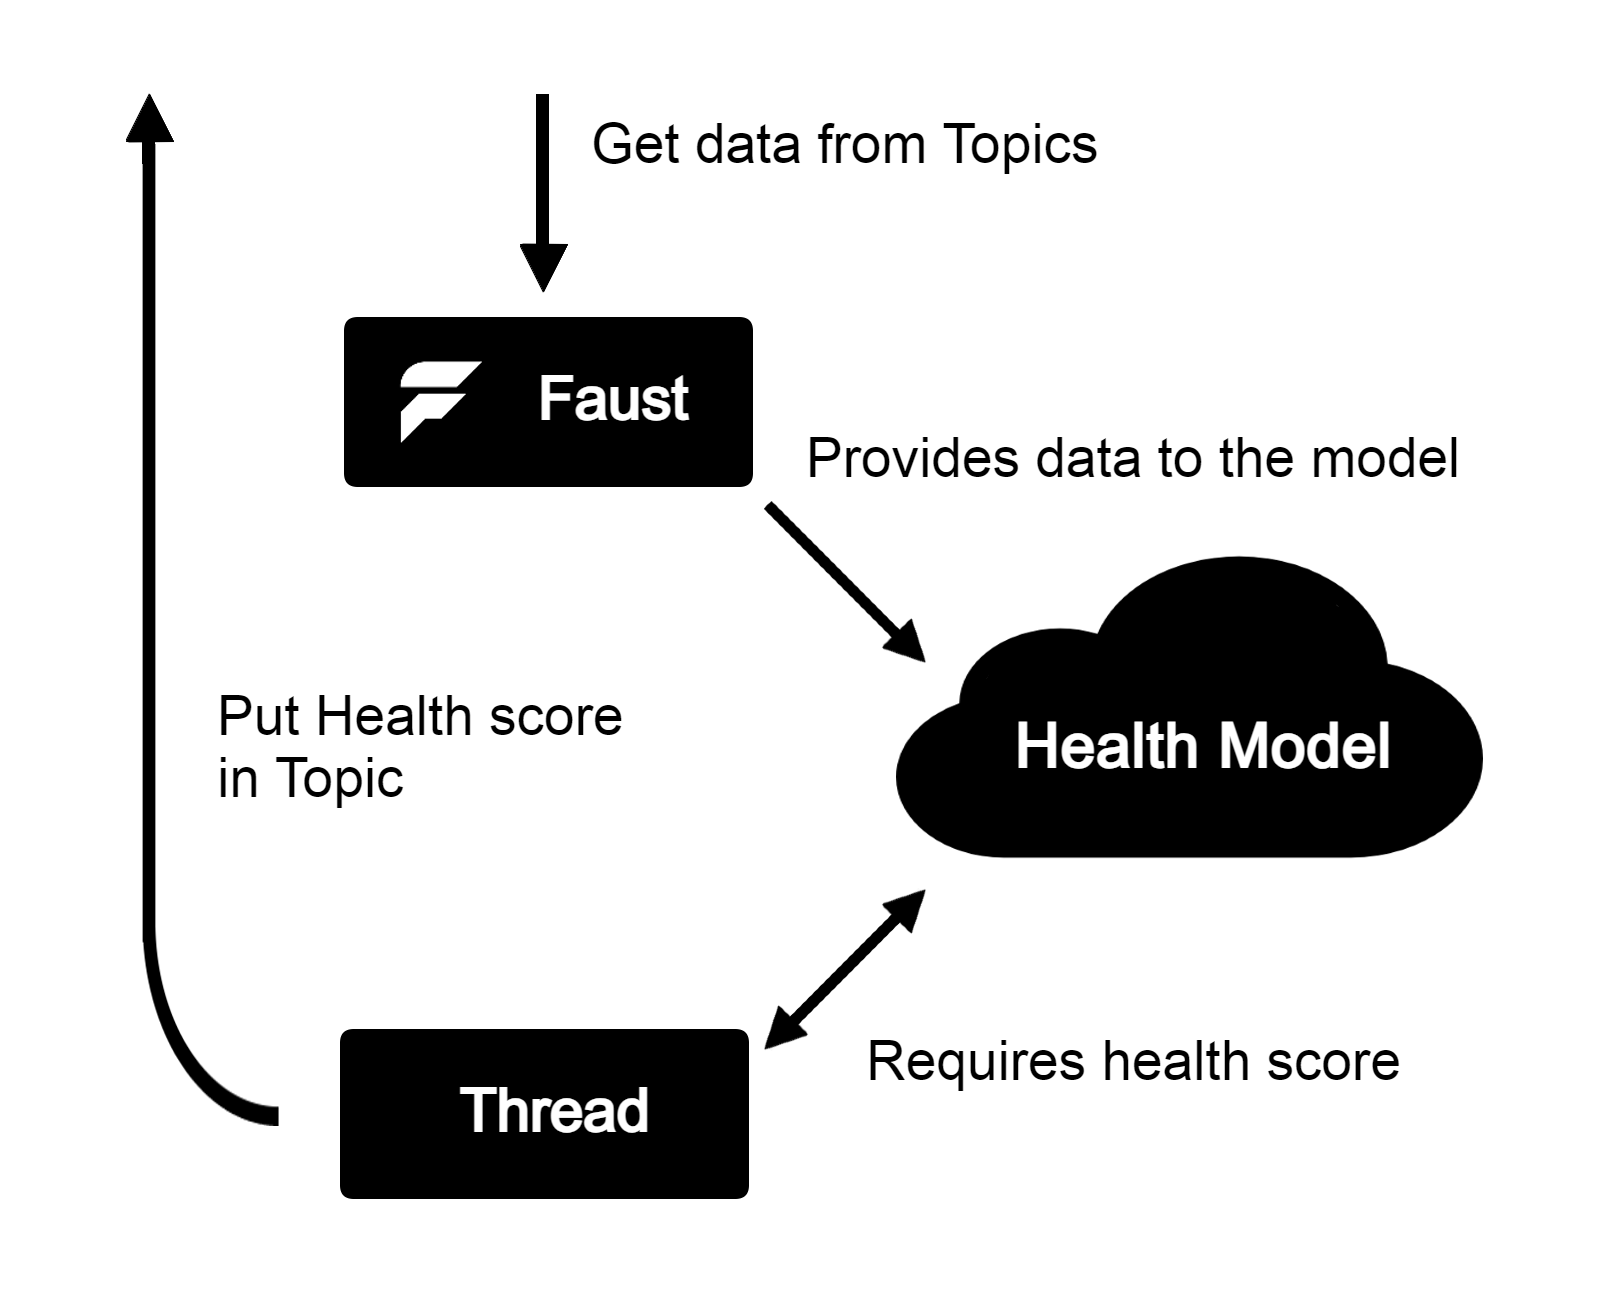
\includegraphics[width=0.8\textwidth]{../Images/SpecificaTecnica/faustFlow.png}
    \caption{Faust Data-flow}
    \label{fig: FaustDataflow}
\end{figure}
In breve:
\begin{enumerate}
    \item Faust ottiene le misurazioni dai topic;
    \item Tramite una porta di accesso le fornisce al modello per il calcolo del punteggio;
    \item Quando l'applicazione Faust viene avviata questa avvia anche un Thread che periodicamente ottiene i punteggi di salute calcolati sulla base delle misurazioni ottenute da Faust e tramite il modulo Writer li invia al topic kafka dedicato.
\end{enumerate}
\subsubsection{Modello per il calcolo del punteggio di salute}
\begin{figure}[H]
    \centering
    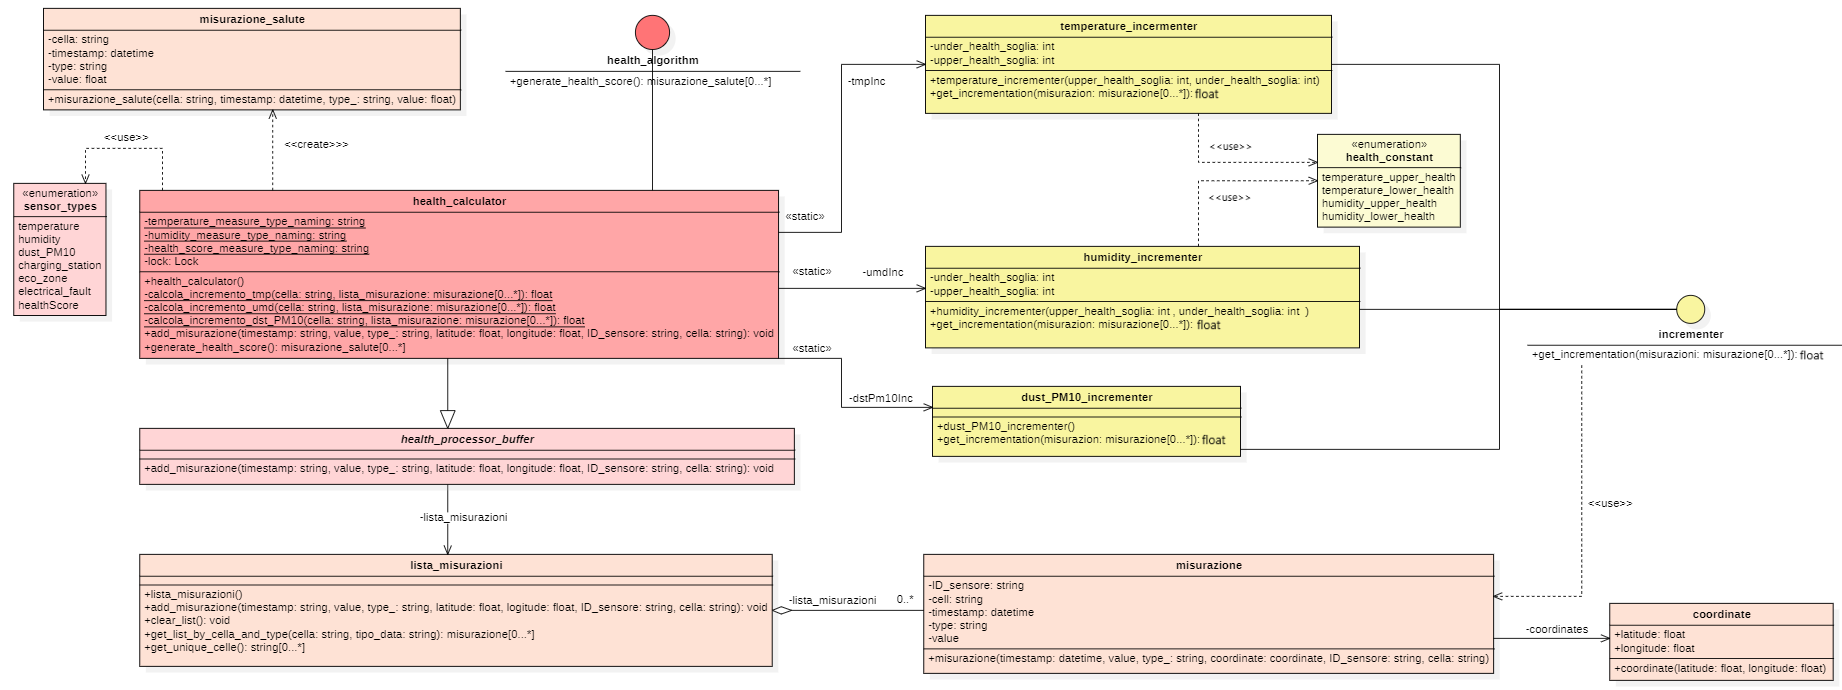
\includegraphics[width=1.1\textwidth]{../Images/SpecificaTecnica/healthModel.PNG}
    \caption{Modello per il calcolo del punteggio di salute - InnovaCity}
    \label{fig: healthModello}
\end{figure}

Il processo per il calcolo del punteggio di salute riceve le letture dei sensori attraverso gli agenti di elaborazione dell'applicazione Faust, i quali sono in ascolto sui topic \textit{Kafka}\textsubscript{\textit{G}} relativi alle misurazioni di temperatura, umidità e polveri sottili PM10. Ad intervalli regolari, il \textit{sistema}\textsubscript{\textit{G}} calcola il punteggio di salute della città basandosi su tali misurazioni. Una volta effettuato il calcolo, il risultato è reso disponibile in un topic \textit{Kafka}\textsubscript{\textit{G}} dedicato.
Il modello che racchiude la logica per il calcolo, richiamato a intervalli regolari, è quello attualmente preso in esame.

In sintesi, il modello:
\begin{itemize}
    \item Riceve le misurazioni di temperatura, umidità e polveri sottili dall'agente dell'app Faust.
    \item Riceve da un thread la richiesta ad intervalli regolari di calcolare i punteggi di salute per le celle della città con le misurazioni ottenute in tempo reale.
\end{itemize}

In accordo con l'\textit{architettura}\textsubscript{\textit{G}} esagonale, la logica del modello è completamente disaccoppiata dai suoi utilizzatori, i quali interagiscono con il modello tramite specifiche classi adapter. Questo approccio promuove la separazione delle preoccupazioni e favorisce la modularità del \textit{sistema}\textsubscript{\textit{G}}. Gli adapter fungono da ponte tra il modello e gli utilizzatori, consentendo una comunicazione fluida e senza dipendenze dirette. Così, eventuali cambiamenti nella logica del modello possono essere implementati senza influenzare gli utilizzatori, garantendo una maggiore flessibilità e manutenibilità del \textit{sistema}\textsubscript{\textit{G}} nel suo complesso.

Il presente modulo è concepito per fornire la logica relativa al puro calcolo del punteggio di salute della città. Tale calcolo si basa su un modello che tiene conto delle misurazioni di temperatura, umidità e polveri sottili PM10. Il modello è stato progettato al fine di determinare un punteggio di salute per ciascuna cella della città in cui sono presenti misurazioni delle suddette tipologie.

\paragraph*{Design Pattern Strategy}

Il modello per il calcolo del punteggio di salute è stato ideato mediante l'utilizzo del design \textit{pattern}\textsubscript{\textit{G}} Strategy. Tale \textit{pattern}\textsubscript{\textit{G}} consente di definire una famiglia di algoritmi, di incapsularli e renderli intercambiabili. Ciò permette di variare l'algoritmo impiegato per il calcolo del punteggio di salute senza incidere sui \textit{processi}\textsubscript{\textit{G}} di elaborazione dell'applicazione Faust o sugli altri componenti del \textit{sistema}\textsubscript{\textit{G}}. In particolare, l'interfaccia \textit{HealthAlgorithm} stabilisce il contratto che deve essere rispettato da tutti gli algoritmi per il calcolo del punteggio di salute.


Inoltre, un'implementazione del \textit{pattern}\textsubscript{\textit{G}} \textit{Strategy} è presente anche negli "Incrementatori". Questi, a partire dalle misurazioni fornite, restituiscono un incremento al punteggio di salute della città. Tale incremento è determinato in base a delle soglie predefinite di temperatura, umidità e polveri sottili PM10, le quali sono definite di default in \textit{health\_constants} ma possono essere impostate al momento della costruzione. In particolare, l'interfaccia \textit{Incrementer} specifica il contratto che deve essere rispettato da tutti gli incrementatori. Vengono implementati tre incrementatori, uno per il calcolo dell'incremento di temperatura, uno per l'umidità e uno per le polveri sottili PM10, come strategie del \textit{pattern}\textsubscript{\textit{G}}.

\paragraph{Classi: metodi e attributi}
\begin{itemize}
    \item{\textbf{Interfaccia: \textit{HealthAlgorithm}}}
    \begin{itemize}
    \item \textbf{Metodi: }
    \begin{itemize}
        \item \textbf{generate\_new\_health\_score(): List[MisurazioneSalute] [abstractmethod]} - Un metodo astratto che deve essere implementato nelle sottoclassi. Questo metodo dovrebbe generare un nuovo punteggio di salute.
    \end{itemize}
    \item\textbf{Note}:
        \begin{itemize}
            \item L'interfaccia definisce il contratto per un algoritmo di salute. Le sottoclassi devono implementare il metodo \textit{generate\_new\_health\_score};
            \item Rappresenta la componente "Strategy" del \textit{pattern}\textsubscript{\textit{G}} omonimo.
            \item Per rispettare il Single responsibility principle, noto anche come principio di coesione, è stata divisa dalla logica di buffering delle misurazioni presente nella classe astratta \textit{HealthProcessorBuffer} poiché l'utilizzatore \textit{HealthCalculatorThread} non utilizza i metodi per il buffering.
        \end{itemize}
    \end{itemize}
    \item\textbf{Classe astratta: \textit{HealthProcessorBuffer}}
    \begin{itemize}
    \item\textbf{Attributi}:
        \begin{itemize}
        \item \textbf{lista\_misurazioni:lista\_misurazioni [private]} - Una lista di oggetti Misurazione.
        \item \textbf{lock:threading.Lock [private]} - Un oggetto lock per gestire l'accesso concorrente alla lista di misurazioni.
    \end{itemize}
    \item \textbf{Metodi: }
    \begin{itemize}
        \item \textbf{add\_misurazione(timestamp, value, type\_, latitude, longitude, ID\_sensore, cella): None [public]} - Aggiunge una nuova misurazione alla lista di misurazioni.
        \item \textbf{clear\_list(): None [public]} - Svuota la lista di misurazioni.
    \end{itemize}
    \item\textbf{Note}:
        \begin{itemize}
               \item La classe astratta definisce un buffer di misurazioni per effettuare il processing su un set di misurazioni. Tale buffer contiene una lista di misurazioni e fornisce metodi per aggiungere misurazioni, ottenere la lista di misurazioni e svuotare la lista.
                \item La logica di buffering e quella dell'algoritmo per il calcolo del punteggio di salute vengono separate in due astrazioni per rispettare il principio di Single Responsibility. Gli utilizzatori di questa classe, i \textit{Processor}, sono interessati esclusivamente al metodo per l'invio del dato al buffer.
                \item La classe astratta definisce un'interfaccia per la comunicazione con gli utilizzatori esterni al modello.
        \end{itemize}
    \end{itemize}
    \item{\textbf{Classe: \textit{HealthCalculator}}}
    \begin{itemize}
    \item\textbf{Attributi}:
        \begin{itemize}
        \item \textbf{tmpInc:TemperatureIncrementer [private]} - Utilizzato per il calcolo dell'incremento di temperatura;
        \item \textbf{umdInc:HumidityIncrementer [private]}; - Utilizzato per il calcolo dell'incremento di umidità;
        \item \textbf{dstPm10Inc:DustPM10Incrementer [private]} - Utilizzato per il calcolo dell'incremento di PM10;
        \item \textbf{temperature\_measure\_type\_naming:string [private]} - Nomenclatura dei tipi di misurazione di temperatura.
        \item \textbf{humidity\_measure\_type\_naming:string [private]} - Nomenclatura dei tipi di misurazione di umidità.
        \item \textbf{ dtsPm10\_measure\_type\_naming:string [private]} - Nomenclatura dei tipi di misurazione di PM10.
        \item \textbf{ healthScore\_measure\_type\_naming:string [private]} - Nomenclatura dei tipi di misurazione di punteggio di salute.
        \item \textbf{lock [private]} - Un oggetto lock per gestire l'accesso concorrente.
    \end{itemize}
    \item \textbf{Metodi: }
    \begin{itemize}
        \item \textbf{generate\_new\_health\_score(): List[MisurazioneSalute] [public]} - Genera e restituisce una nuova lista di punteggi di salute, uno per ogni cella della città di cui sono state fornite misurazioni.
        \item \textbf{calcola\_incremento\_tmp(cella: str, lista\_misurazioni): int [private]} - Calcola e restituisce l'incremento della temperatura.
        \item \textbf{calcola\_incremento\_umd(cella: str, lista\_misurazioni): int [private]} - Calcola e restituisce l'incremento dell'umidità.
        \item \textbf{calcola\_incremento\_dstPm10(cella: str, lista\_misurazioni): int [private]} - Calcola e restituisce l'incremento della polvere PM10.
    \end{itemize}
    \item\textbf{Note}:
        \begin{itemize}
            \item La classe implementa l'interfaccia \textit{HealthAlgorithm} e la classe astratta \textit{HealthProcessorBuffer} per calcolare il punteggio di salute tramite la strategia concreta definita in \textit{generate\_new\_health\_score()} che genera una nuova lista di punteggi di salute.
            \item Questa classe rappresenta il vero cervello del calcolo del punteggio di salute in quanto utilizzatore di tutti gli incrementatori e delle misurazioni bufferizzate per creare una strategia di calcolo.
        \end{itemize}
    \end{itemize}
    \item\textbf{Classe: \textit{Misurazione}}
    \begin{itemize}
        \item   \textbf{Attributi}: 
    \begin{itemize}
        \item \textbf{timestamp:datetime [private]} - Timestamp della misurazione.
        \item \textbf{value:T [private]} - Valore della misurazione.
        \item \textbf{type:str [private]} - Tipo della misurazione.
        \item \textbf{coordinates:coordinate [private]} - Coordinate della misurazione.
        \item \textbf{ID\_sensore:str [private]} - \textit{ID}\textsubscript{\textit{G}} del \textit{sensore}\textsubscript{\textit{G}} che ha effettuato la misurazione.
        \item \textbf{cella:str [private]} - Cella in cui è stata effettuata la misurazione.
    \end{itemize}
    \item   \textbf{Metodi}: 
    \begin{itemize}
        \item \textbf{\_\_eq\_\_(other:Misurazione):bool [public]} - Ridefinizione dell'operatore di uguaglianza per confrontare due oggetti Misurazione.
    \end{itemize}
\end{itemize}
    \item\textbf{Classe: \textit{coordinate}}
    \begin{itemize}
        \item    \textbf{Attributi}: 
    \begin{itemize}
        \item \textbf{latitude:float [private]} - Latitudine della coordinata.
        \item \textbf{longitude:float [private]} - Longitudine della coordinata.
    \end{itemize}
    \item     \textbf{Metodi}: 
    \begin{itemize}
        \item \textbf{\_\_eq\_\_(other:coordinate):bool [public]} - Ridefinizione dell'operatore di uguaglianza per confrontare due oggetti Coordinate.
    \end{itemize}
\end{itemize}
\item\textbf{Classe: \textit{MisurazioneSalute}}
    \begin{itemize}
    \item\textbf{Attributi}:
        \begin{itemize}
        \item \textbf{timestamp:datetime [private]} - Il timestamp della misurazione di salute.
        \item \textbf{value:float [private]} - Il valore della misurazione di salute.
        \item \textbf{type:string [private]} - Il tipo della misurazione.
        \item \textbf{cella:string [private]} - La cella della misurazione di salute.
    \end{itemize}
    \item\textbf{Note}:
        \begin{itemize}
            \item La classe rappresenta una misurazione di salute. Contiene informazioni sul timestamp, il valore (ovvero il punteggio di salute calcolato), il tipo della misurazione e la cella relativa alla misurazione.
        \end{itemize}
    \end{itemize}
    \item\textbf{Classe: \textit{lista\_misurazioni}}
    \begin{itemize}
    \item\textbf{Attributi}:
        \begin{itemize}
        \item \textbf{list:List[Misurazione] [private]} - Una lista di oggetti Misurazione.
    \end{itemize}
    \item \textbf{Metodi: }
    \begin{itemize}
        \item \textbf{add\_misurazione(timestamp, value, type\_, latitude, longitude, ID\_sensore, cella): None [public]} - Aggiunge una nuova misurazione alla lista.
        \item \textbf{clear\_list(): None [public]} - Svuota la lista di misurazioni.
        \item \textbf{get\_list\_by\_cella\_and\_type(cella: str, tipo\_dato: str): List[Misurazione] [public]} - Restituisce una lista di misurazioni che corrispondono alla cella e al tipo di misurazione specificati (temperatura,umidità,ecc.).
        \item \textbf{get\_unique\_celle(): List[str] [public]} - Restituisce la lista di celle presenti nelle misurazioni senza ripetzioni.
    \end{itemize}
    \item\textbf{Note}:
        \begin{itemize}
            \item La classe rappresenta una lista di misurazioni. Fornisce metodi per aggiungere misurazioni, svuotare la lista, ottenere misurazioni per cella e tipo di misurazioni, e ottenere le celle di cui si hanno misurazioni.
        \end{itemize}
    \end{itemize}
    \item\textbf{Enumerazione: \textit{SensorTypes}}
        \begin{itemize}
            \item \textbf{Costanti}: 
            \begin{itemize}
                \item \textbf{TEMPERATURE:str [public]} - Rappresenta la nomenclatura dei \textit{sensore}\textsubscript{\textit{G}} di temperatura.
                \item \textbf{HUMIDITY:str [public]} - Rappresenta la nomenclatura dei \textit{sensore}\textsubscript{\textit{G}} di umidità.
                \item \textbf{DUST\_PM10:str [public]} - Rappresenta la nomenclatura dei \textit{sensore}\textsubscript{\textit{G}} di "polvere PM10".
                \item \textbf{CHARGING\_STATION:str [public]} - Rappresenta la nomenclatura dei \textit{sensore}\textsubscript{\textit{G}} di stato delle colonnine di ricarica.
                \item \textbf{ECOLOGICAL\_ISLAND:str [public]} - Rappresenta la nomenclatura dei \textit{sensore}\textsubscript{\textit{G}} di stato riempimento isole ecologica.
                \item \textbf{WATER\_PRESENCE:str [public]} - Rappresenta la nomenclatura dei \textit{sensore}\textsubscript{\textit{G}} di presenza d'acqua.
                \item \textbf{ELECTRICAL\_FAULT:str [public]} - Rappresenta la nomenclatura dei \textit{sensore}\textsubscript{\textit{G}} di guasti elettrici.
            \end{itemize}

            \item \textbf{Note}:
            \begin{itemize}
                \item L'enumerazione viene utilizzata per centralizzare la gestione della nomenclatura dei tipi di sensori che verrà salvata nelle misurazioni.
            \end{itemize}
        \end{itemize}
\item \textbf{Interfaccia: \textit{Incrementer}}
    \begin{itemize}
    \item \textbf{Metodi: }
    \begin{itemize}
        \item \textbf{get\_incrementation(misurazioni: List[Misurazione]): int [abstractmethod]} - Un metodo astratto che deve essere implementato nelle sottoclassi. Questo metodo calcola e restituire un incremento basato sulla lista di misurazioni fornita.
    \end{itemize}
    \item\textbf{Note}:
        \begin{itemize}
            \item L'interfaccia definisce il contratto per un incrementatore. Le sottoclassi devono implementare il metodo \textit{get\_incrementation()}.
            \item Rappresenta la componente "Strategy" del \textit{pattern}\textsubscript{\textit{G}} omonimo.
        \end{itemize}
    \end{itemize}
    \item \textbf{Classe: \textit{TemperatureIncrementer}}
    \begin{itemize}
    \item \textbf{Attributi}:
        \begin{itemize}
        \item \textbf{upper\_health\_soglia:int [private]} - La soglia superiore di benessere per la temperatura;
        \item \textbf{under\_health\_soglia:int [private]} - La soglia inferiore di benessere per la temperatura.
    \end{itemize}
    \item \textbf{Metodi: }
    \begin{itemize}
        \item \textbf{get\_incrementation(misurazioni: List[Misurazione]): int [public]} - Calcola e restituisce un incremento basato sulle sole misurazioni di temperatura della lista fornita.
    \end{itemize}
    \item\textbf{Note}:
        \begin{itemize}
            \item La classe implementa l'interfaccia \textit{Incrementer};
            \item I valori di default per le soglie vengono presi dall'enumerazione \textit{HealthConstant} altrimenti sono impostabili alla costruzione.
            \item Rappresenta una strategia concreta del \textit{pattern}\textsubscript{\textit{G}} \textit{Strategy} per il calcolo dell'incremento di temperatura.
        \end{itemize}
    \end{itemize}
    \item{\textbf{Classe: \textit{HumidityIncrementer}}}
    \begin{itemize}
    \item\textbf{Attributi}:
        \begin{itemize}
        \item \textbf{upper\_health\_soglia:int [private]} - La soglia superiore di benessere per l'umidità;
        \item \textbf{under\_health\_soglia:int [private]} - La soglia inferiore di benessere per l'umidità.
    \end{itemize}
    \item \textbf{Metodi: }
    \begin{itemize}
        \item \textbf{get\_incrementation(misurazioni: List[Misurazione]): int [public]} - Calcola e restituisce un incremento basato sulle sole misurazioni di umidità della lista fornita.
    \end{itemize}
    \item\textbf{Note}:
        \begin{itemize}
            \item La classe implementa l'interfaccia \textit{Incrementer};
            \item I valori di default per le soglie vengono presi dall'enumerazione \textit{HealthConstant} altrimenti sono impostabili alla costruzione.
            \item Rappresenta una strategia concreta del \textit{pattern}\textsubscript{\textit{G}} \textit{Strategy} per il calcolo dell'incremento di umidità.
        \end{itemize}
    \end{itemize}\item{\textbf{Classe: \textit{DustPM10Incrementer}}}
    \begin{itemize}
    \item \textbf{Metodi: } 
    \begin{itemize}
        \item \textbf{get\_incrementation(misurazioni: List[Misurazione]): int [public]} - Calcola e restituisce un incremento basato sulle sole misurazioni di polveri sottili della lista fornita.
    \end{itemize}
    \item\textbf{Note}:
        \begin{itemize}
            \item La classe implementa l'interfaccia \textit{Incrementer};
            \item Rappresenta una strategia concreta del \textit{pattern}\textsubscript{\textit{G}} \textit{Strategy} per il calcolo dell'incremento di polveri sottili PM10.
            \item A differenza degli altri \textit{Incrementer}, \textit{DustPM10Incrementer} non definisce soglie di benessere in quanto è scontato che il valore ottimale di inquinamento è zero.
        \end{itemize}
    \end{itemize}

\end{itemize}

\subsubsection{Modulo Writer}
\begin{figure}[H]
    \centering
    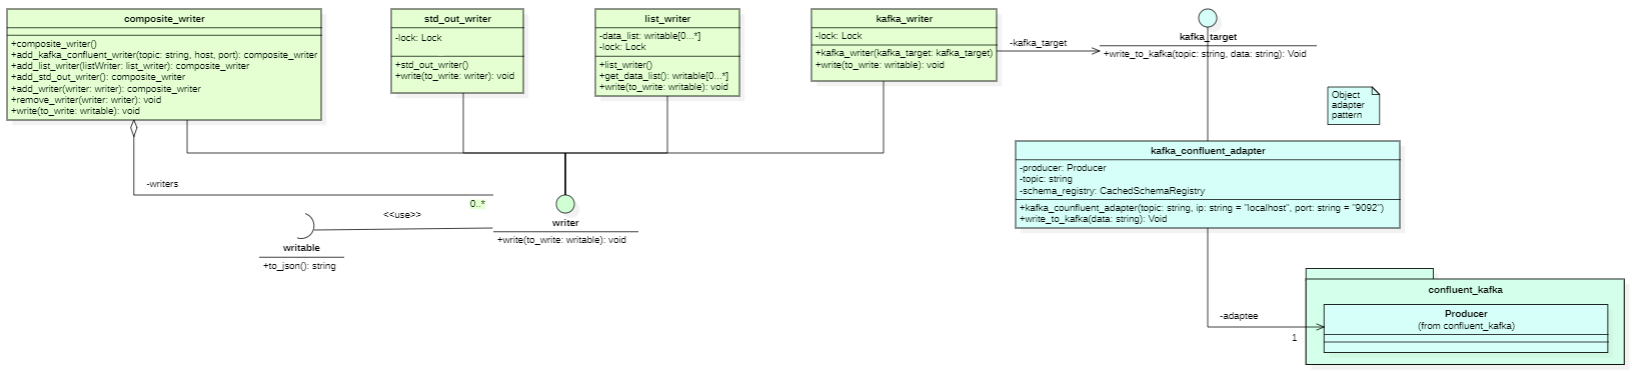
\includegraphics[width=1\textwidth]{../Images/SpecificaTecnica/writerModule.PNG}
    \caption{Modulo Writer - InnovaCity}
    \label{fig: healthModelloWriter}
\end{figure}
Il modulo Writer è lo stesso di quello descritto in \ref*{sec:writersModule} e viene nella sua totalità riutilizzato per la scrittura dei punteggi di salute calcolati.
Non viene riportata la strategia di scrittura su di una lista poichè non ne è stato ritenuto necessario l'utilizzo.

\paragraph*{Classi: metodi e attributi}
Tutte le informazioni sono già state esposte in: \ref*{sec:writersModule}.

\subsubsection{Modulo Threading/Scheduling}
\begin{figure}[H]
    \centering
    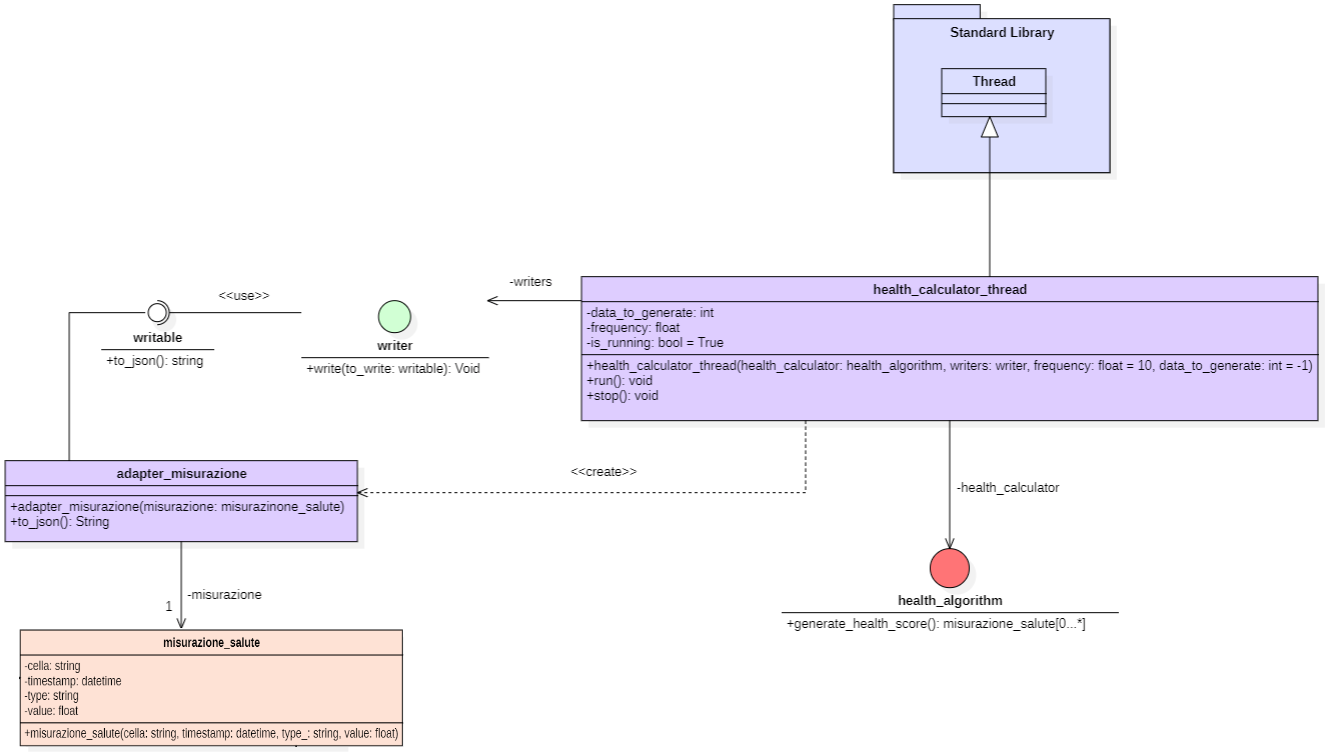
\includegraphics[width=1\textwidth]{../Images/SpecificaTecnica/healthThreading.PNG}
    \caption{Modulo Threading/Scheduling health Model - InnovaCity}
    \label{fig: threadHealth}
\end{figure}

Questo modulo si occupa di integrare la logica di Scheduling e Threading per il calcolo periodico del punteggio di salute della città e quella di scrittura/invio di \textit{Writable}. In particolare, fornisce un'implementazione di un thread che, a intervalli regolari, richiama il calcolo del punteggio di salute della città. Successivamente, utilizzando il modulo "Writer", adatta le misurazioni di salute ottenute all'interfaccia per renderle un oggetto che implementa \textit{Writable}. Pertanto, questo modulo è utilizzatore del modello per il calcolo del punteggio di salute e del modulo di Writer.
In sintesi, il modulo:
    \begin{enumerate}
        \item Richiama l'algoritmo per calcolo del punteggio di salute della città a intervalli regolari;
        \item Scrive il risultato ottenuto sul topic \textit{Kafka}\textsubscript{\textit{G}} dedicato.
    \end{enumerate}

\paragraph*{Dependecy Inversion principle}
Il modulo di scheduling e threading dipende dall'astrazione dell'interfaccia del modello per il calcolo del punteggio di salute e del modulo di Writer, invece di dipendere direttamente dalle implementazioni concrete di questi moduli. Ciò consente una maggiore flessibilità e facilità di manutenzione, poiché il modulo di scheduling e threading non è vincolato a implementazioni specifiche, ma può essere facilmente adattato per utilizzare diverse implementazioni che soddisfano lo stesso contratto.

In sostanza, seguendo il principio di Inversione delle Dipendenze, il modulo di scheduling e threading si concentra sull'utilizzo di interfacce o astrazioni, piuttosto che sulle implementazioni concrete, rendendo il \textit{sistema}\textsubscript{\textit{G}} più modulare, scalabile e facilmente estendibile.

\paragraph*{Classi: metodi e attributi}
\begin{itemize}
    \item{\textbf{Classe: \textit{HealthCalculatorThread}}}
    \begin{itemize}
    \item\textbf{Attributi}:
        \begin{itemize}
        \item \textbf{healthCalculator: HealthAlgorithm [private]} - Un implementatazione dell'interfaccia \textit{HealthAlgorithm}, ovvero una strategia per il calcolo del punteggio.
        \item \textbf{frequency: float [private]} - La frequenza con cui il thread genera nuovi punteggi di salute.
        \item \textbf{is\_running: bool [private]} - Un flag che indica se il thread è in esecuzione.
        \item \textbf{data\_to\_generate: int [private]} - Il numero di misurazioni di salute da generare.
        \item \textbf{writers: Writer [private]} - Un oggetto della classe Writer. (Singolo scrittore o albero, Composite \textit{pattern}\textsubscript{\textit{G}})
    \end{itemize}
    \item \textbf{Metodi: }
    \begin{itemize}
        \item \textbf{run(): None [public]} - Esegue il thread, generando nuovi punteggi di salute a una certa frequenza.
        \item \textbf{stop(): None [public]} - Ferma l'esecuzione del thread.
    \end{itemize}
    \item\textbf{Note}:
        \begin{itemize}
            \item La classe estende la classe \textit{threading.Thread}.
            \item Se \textit{data\_to\_generate} è < 0 genera misurazioni di salute finchè il thread non viene interroto dall'esterno.
            \item   Grazie al \textit{pattern}\textsubscript{\textit{G}} \textit{Strategy} è possibile cambiare agevolmente l'algoritmo volto al calcolo del punteggio di salute della città.
        \end{itemize}
    \end{itemize}
\end{itemize}

\subsubsection{Modulo Processing}
\begin{figure}[H]
    \centering
    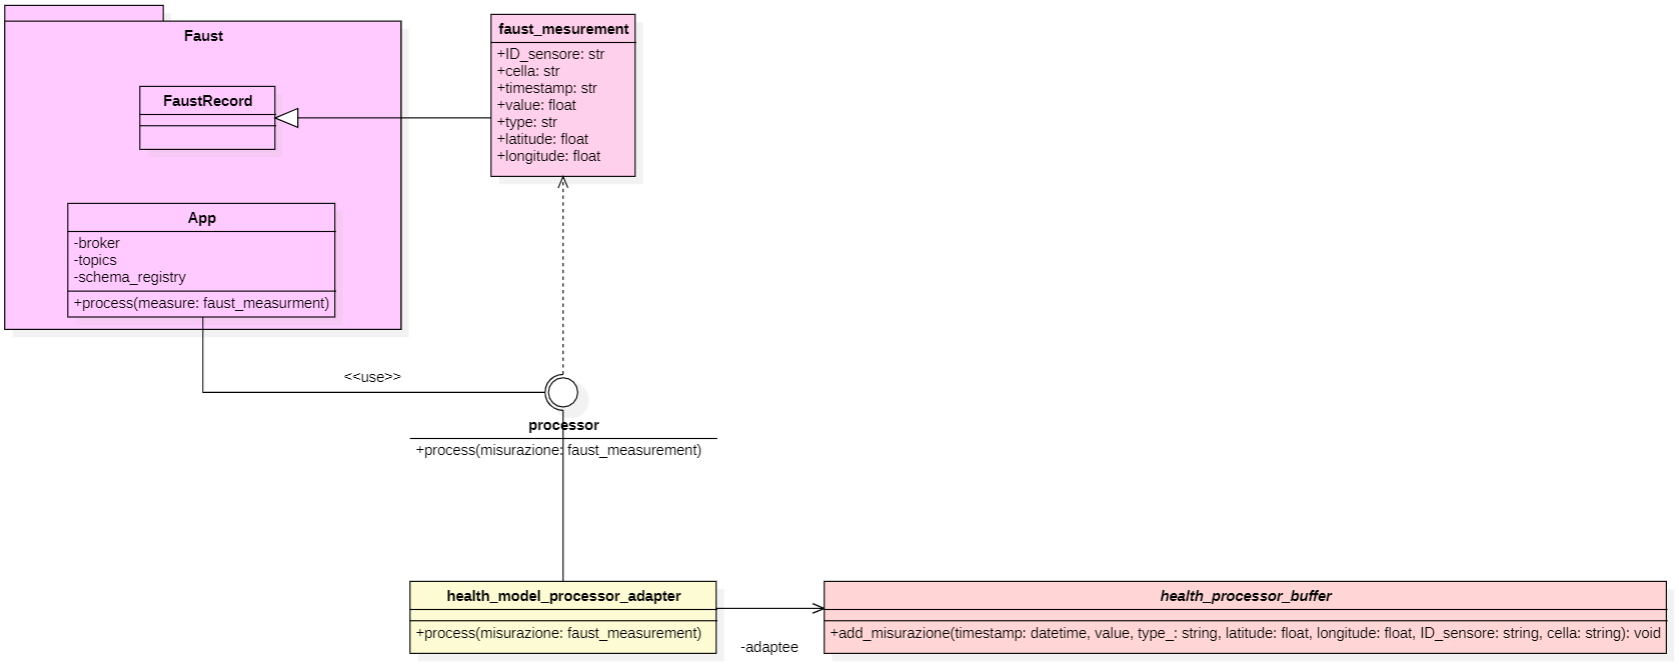
\includegraphics[width=1\textwidth]{../Images/SpecificaTecnica/processorFaust.PNG}
    \caption{Modulo Processing - InnovaCity}
    \label{fig: processHealth}
\end{figure}
Per garantire un'interfaccia uniforme per i metodi di elaborazione dei dati provenienti da \textit{Kafka}\textsubscript{\textit{G}} tramite Faust e per stabilire un canale di comunicazione con il modello per il calcolo del punteggio di salute, viene sviluppato il modulo di Processing. Questo modulo offre l'interfaccia target denominata \textit{Processor}, e un adapter a \textit{Processor} per l'invio delle misurazioni al modello per il calcolo del punteggio di salute, denominato \textit{HealthModelProcessorAdapter}.

\paragraph*{Design Pattern Object Adapter}
Nel contesto dell'applicazione Faust, all'interno del ruolo svolto dagli agenti, ogni volta che una misurazione viene ricevuta, viene invocato il metodo \textit{process\_measure()} dell'implementazione dell'interfaccia \textit{Processor}, denominata \textit{HealthModelProcessorAdapter}. In particolare, \textit{HealthModelProcessorAdapter} adatta la classe astratta \textit{HealthModelBuffer}, che rappresenta un buffer di misurazioni utilizzato per eseguire il calcolo periodico del punteggio di salute della città, all'interfaccia \textit{Processor}.

Questo \textit{pattern}\textsubscript{\textit{G}} consente di incapsulare le logiche di elaborazione e di rendere il modello indipendente dall'implementazione specifica dell'applicazione Faust. Allo stesso tempo, facilita la sostituzione dell'operazione di elaborazione eseguita su ogni misurazione dagli agenti grazie al contratto dell'interfaccia \textit{Processor}.
\paragraph*{Classi: metodi e attributi}
\begin{itemize}
    \item{\textbf{Interfaccia: \textit{Processor}}}
    \begin{itemize}
    \item\textbf{Metodi: }
    \begin{itemize}
        \item \textbf{process(misurazione: FaustMeasurement): None [public, abstract]} - Un metodo astratto che deve essere implementato nelle sottoclassi. Questo metodo elabora una misurazione.
    \end{itemize}
    \item\textbf{Note}:
        \begin{itemize}
            \item  Le sottoclassi devono implementare il metodo astratto \textit{process()} definendo la propria operazione da effettuare su ogni misurazione ricevuta dai topic di iscrizione.
            \item Rappresenta la componente "Target" del \textit{pattern}\textsubscript{\textit{G}} \textit{Object Adapter}.
            \item L'interfaccia è stata progettata per garantire un'interfaccia uniforme per i metodi di elaborazione dei dati provenienti da \textit{Kafka}\textsubscript{\textit{G}} tramite Faust.
            \item Rappresenta un contratto per l'elaborazione di misurazioni.
            \item Gli agenti in ascolto sul topic utilizzeranno un implementatazione di \textit{Processor} per effettuare l'elaborazione delle misurazioni ottenute.
        \end{itemize}
    \end{itemize}
    \item{\textbf{Classe: \textit{FaustMeasurement}}}
    \begin{itemize}
    \item\textbf{Attributi}:
        \begin{itemize}
        \item \textbf{timestamp: str} - Il timestamp della misurazione.
        \item \textbf{value: float} - Il valore della misurazione.
        \item \textbf{type: str} - Il tipo della misurazione.
        \item \textbf{latitude: float} - La latitudine della misurazione.
        \item \textbf{longitude: float} - La longitudine della misurazione.
        \item \textbf{ID\_sensore: str} - L'\textit{ID}\textsubscript{\textit{G}} del \textit{sensore}\textsubscript{\textit{G}} che ha effettuato la misurazione.
        \item \textbf{cella: str} - La cella della misurazione.
    \end{itemize}
    \item\textbf{Note}:
        \begin{itemize}
            \item La classe \textit{FaustMeasurement} definita utilizzando \textit{faust.Record} rappresenta un singolo record di misurazione proveniente da un \textit{sensore}\textsubscript{\textit{G}} in un'applicazione Faust basata su \textit{Python}\textsubscript{\textit{G}}
            \item Faust si occupa automaticamente della conversione dei dati in formato JSON in base agli attributi definiti, facilitando la trasmissione e la ricezione dei dati nei topic \textit{Kafka}\textsubscript{\textit{G}}.
            \item È possibile definire la validazione dei dati in ingresso per garantire l'integrità e la coerenza delle misurazioni.
            \item \textbf{In sintesi}:
            Questa classe viene utilizzata in un'applicazione Faust per definire il tipo di dati atteso nei topic \textit{Kafka}\textsubscript{\textit{G}}. I dati provenienti dai sensori, contenenti timestamp, valore, tipo, coordinate geografiche, identificativo del \textit{sensore}\textsubscript{\textit{G}} e eventuale cella di appartenenza, verranno convertiti in oggetti di tipo FaustMeasurement prima di essere elaborati dall'applicazione.
        \end{itemize}
    \end{itemize}
    \item{\textbf{Classe: \textit{HealthModelProcessorAdapter}}}
    \begin{itemize}
    \item\textbf{Attributi}:
        \begin{itemize}
        \item \textbf{healthCalculator: HealthProcessorBuffer} - Un implementazione di HealthProcessorBuffer.
    \end{itemize}
    \item \textbf{Metodi: }
    \begin{itemize}
        \item \textbf{process(misurazione: FaustMeasurement): None [public, async]} - Aggiunge la misurazione all'oggetto \textit{HealthProcessorBuffer} adattando \textit{FaustMeasurement} alla porta di accesso fornita da \textit{HealthProcessorBuffer} per l'elaborazione volta al calcolo del punteggio di salute.
    \end{itemize}
    \item\textbf{Note}:
        \begin{itemize}
            \item La classe implementa l'interfaccia \textit{Processor}. Implementa il metodo astratto \textit{process()} per aggiungere/adattare la misurazione del tipo \textit{FaustMeasurement} ad un implementatazione di \textit{HealthProcessorBuffer}.
            \item Rappresenta la componente "Adapter" del \textit{pattern}\textsubscript{\textit{G}} \textit{Object Adapter}.
        \end{itemize}
    \end{itemize}
\end{itemize}